\chapter{Counting}

\section{Counting be like}
But Brandon, I hear your thoughts again. \\
Why in the holy Spaghetti Monster Shall we learn how to count?

The ``counting'' we address here in a discrete mathematical sense is not about counting from number to number in an arithmetic sequence. It's about estimating the number of possibilities. \\
For instance, consider a deck of 40 cards. What is the probability from which you draw all 5 parts of the inexorable Exodia? What is the total number of cases about the combination of 5 cards you draw from your deck, and from there within, what are all possible cases of drawing five cards of some same category (number 8, club, diamond...)? \\
Most importantly, what is the probability of it? \\
The techniques we employ to estimate and learn the total number of possible cases according to some conditions is known as \textbf{counting}. \\
In this chapter, let us begin from counting in simpler circumstances, like counting sequences.

\subsection{Counting Sequences}
Let there be a set $S = \{1, 2, \cdots, n\}$. \\
We may pick $k \leq n$ elements from this set $S$, one at a time, while removing what we have sampled (selected) from $S$. This is known as \textbf{sampling without replacement}: once we select something from a set, it is removed from the set. \\
When counting the number of different ways to do this, either order matters, or order doesn't. In the case that order does matter, we are counting ordered sequences.

The most daily-life example would be Poker (without money, that's the relevant part .-.). \\
When we deal a card, that card dissappears is sampled from, as well as removed the deck. Meanwhile, when the sequence is ordered, the sequence of dealing card A then card B is different from the sequence of dealing card B then card A. \\
Therefore, at the first card, we have 52 disctinct possibilities for the card we now deal. \\
The second card, however, depends on the first card, since it cannot coincide with the first card. Your hand cannot have two exactly same card. That is cheating, and COMPSCI 70 does not condone cheating. \\
This means the second card has 51 possible choices, whichever card we picked from the first. Notice again that albeit the number of possibilities is the same, the second card you can get comes from a different set of cards depending on your first card.

Therefore, the total amount of possibilities for drawing 5 cards from a 52-card poker deck is in fact:
\[52 \times (52 - 1) \times (52 - 2) \times (52 - 3) \times (52 - 4)\]
This brings us to the \textbf{First Rule of Counting}:
\begin{ln-axiom}{The First Rule of Counting}{}
    If an object can be made by a sucession of $k$ choices, where there are $n_i$ ways to make the $i^{th}$ choice, then the total number of distinct objects that can be made in this way is:
    \[\pi_{i = 1}^k n_i\]
\end{ln-axiom}

Let us use this opportunity to introduce another instinct:
\begin{ln-fig}{The Tree of Counting}{}
    \begin{center}
        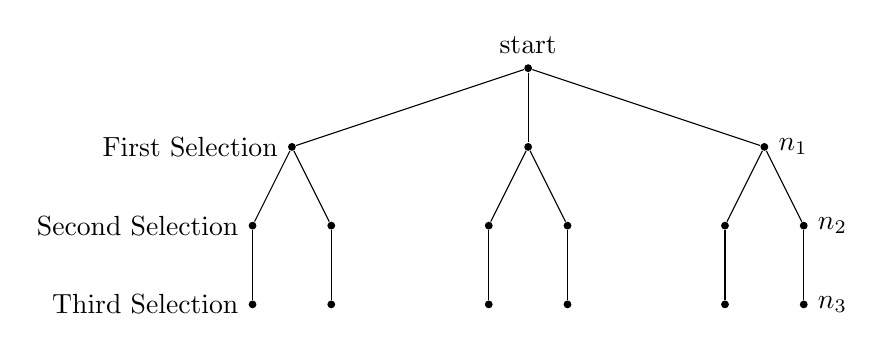
\begin{tikzpicture}
            [point/.style = {circle, fill, inner sep = 1pt}]
            \node[point] (1a) [label=above:start] at (6.5, 3) {};
            \node[point] (2a) [label=left:\text{First Selection}] at (3.5, 2) {};
            \node[point] (2b) at (6.5, 2) {};
            \node[point] (2c) [label=right:$n_1$] at (9.5, 2) {};
            \node[point] (3a) [label=left:\text{Second Selection}] at (3, 1) {};
            \node[point] (3b) at (4, 1) {};
            \node[point] (3c) at (6, 1) {};
            \node[point] (3d) at (7, 1) {};
            \node[point] (3e) at (9, 1) {};
            \node[point] (3f) [label=right:$n_2$] at (10, 1) {};
            \node[point] (4a) [label=left:\text{Third Selection}] at (3, 0) {};
            \node[point] (4b) at (4, 0) {};
            \node[point] (4c) at (6, 0) {};
            \node[point] (4d) at (7, 0) {};
            \node[point] (4e) at (9, 0) {};
            \node[point] (4f) [label=right:$n_3$] at (10, 0) {};
            \draw (1a) -- (2a);
            \draw (1a) -- (2b);
            \draw (1a) -- (2c);
            \draw (2a) -- (3a);
            \draw (2a) -- (3b);
            \draw (2b) -- (3c);
            \draw (2b) -- (3d);
            \draw (2c) -- (3e);
            \draw (2c) -- (3f);
            \draw (3a) -- (4a);
            \draw (3b) -- (4b);
            \draw (3c) -- (4c);
            \draw (3d) -- (4d);
            \draw (3e) -- (4e);
            \draw (3f) -- (4f);
        \end{tikzpicture}
    \end{center}
\end{ln-fig}
Say we are looking for the number of ordered sequences produced from sampling from a three-card deck. Then, we will once again have 3 possibilities for the first card, 2 for the second card, and 1 for the third card (provided it's the last card chosen). \\
In the above figure, each leaf node is a termination of the sampling process: a possibility. Therefore, we just count the number of leaf nodes that exist in this tree: in this case:
\[n_1 \times n_2 \times n_3 = 3 \times 2 \times 1 = 6\]

\subsection{Counting Sets}
Sets are slightly different stories from sequences, since there is no order in set. \\
Put in a deck drawing context as discussed in prior subsection, we would then be counting the number of distinct hands: where hands do not all have same members (cards). \\
To count the distinct subsets of a set $S$ (in this case our deck) with $5$ cards, we can let each sequence get placed into some bin corresponding to the set of 5 elements in the sequence. Each bin must contain $5!$ ways of ordering the $5$ elements in the set. \\
This means we just have to find the number of bins (distinct sets), which is essentially dividing the number of ordered sequences with $5!$ for this context:
\[\frac{52!}{(52 - 5)!5!}\]
This quantity, $\frac{n!}{(n - k)!k!}$, stands for the number of $k$-element subsets from an n-element set $S$, the result of our counting. The alternative but more popular expression of this is $\binom{n}{k}$:
\begin{ln-theorem}{Second Rule of Counting}{}
    Assume an object is made by a succession of choices, and the order in which the choices are made does not matter. \\
    Let $A$ be the set of ordered objects, $B$ the set of unordered objects. If there exists an $m-to-1$ function $f: A \rightarrow B$, then we can count the number of ordered objects and divide by $m$ to obtain the number of unordered objects.
\end{ln-theorem}
So in the hand-counting context of this subsection, we had a $5!$-to-$1$ function from set of all ordered sequences to set of all distinct hands (which are the unordered sequences we count for).

\section{Sampling with Replacement}
Sampling with replacement is another different scenario of sampling we'd like to consider. \\
Perhaps the most daily-life example would be gacha games, where in each trial players have a constant probability of obtaining a specific in-game item. \\
To avoid counterarguments: if your game doesn't have constant probability and is also not sampling without replacement, it's a third type of scenario where we have a separate probability model and is not simplistic enough for the scope of this section. I don't know, you may have played the wrong game. \\
But perhaps, a slightly more relatable example would have been tossing coins. In each coin toss, the only two possible results are heads and tails. You can sample a head, but cannot remove the possibility of rolling a head from the total possible consequences of tossing a coin. Therefore, this is sampling with replacement. \\
I also don't want to talk about instances where your coin does not land on head or tails. As COMPSCI 70 emphasize, we do not condone cheating.

What are the mathematical properties of sampling with replacement? \\
Well, since no elements are removed from $S$, the number of possible choices across each selection will be constant, provided that the numebr of elements in $S$ is always constant and does not decrease. \\
Since we have $n$ choices in each trial, across $k$ selections in the process of creating a $k$-length sequence, 
\[n_1 = n_2 = \cdots = n_k = n\]
Therefore, the total number of possible ordered $k$-length sequences from an $n$-element set $S$ under sample with replacement is $n^k$.

\subsection{Here is an Example}
We may visit coin tosses first. The total possible outcomes of tossing a coin $k=3$ times can be portrayed by the following tree:
\begin{ln-fig}{The Tree of Counting on Coins}{}
    \begin{center}
        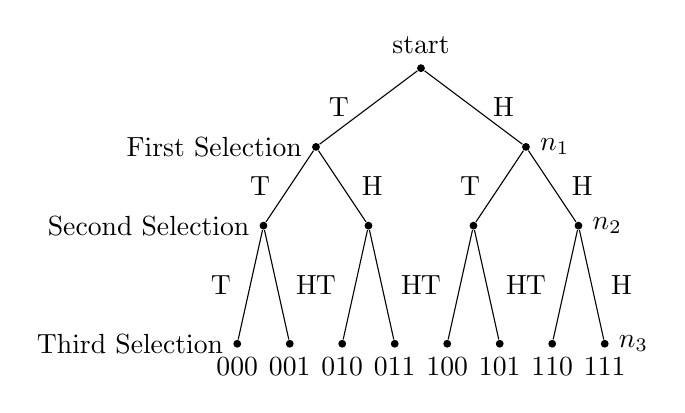
\begin{tikzpicture}
            [point/.style = {circle, fill, inner sep = 1pt}]
            \node[point] (1a) [label=above:start] at (7/3, 3) {};
            \node[point] (2a) [label=left:\text{First Selection}] at (3/3, 2) {};
            \node[point] (2b) [label=right:$n_1$] at (11/3, 2) {};
            \node[point] (3a) [label=left:\text{Second Selection}] at (1/3, 1) {};
            \node[point] (3b) at (5/3, 1) {};
            \node[point] (3c) at (9/3, 1) {};
            \node[point] (3d) [label=right:$n_2$] at (13/3, 1) {};
            \node[point] (4a) [label=left:\text{Third Selection}, label=below:$000$] at (0, -0.5) {};
            \node[point] (4b) [label=below:$001$] at (2/3, -0.5) {};
            \node[point] (4c) [label=below:$010$] at (4/3, -0.5) {};
            \node[point] (4d) [label=below:$011$] at (6/3, -0.5) {};
            \node[point] (4e) [label=below:$100$] at (8/3, -0.5) {};
            \node[point] (4f) [label=below:$101$] at (10/3, -0.5) {};
            \node[point] (4g) [label=below:$110$] at (12/3, -0.5) {};
            \node[point] (4h) [label=right:$n_3$, label=below:$111$] at (14/3, -0.5) {};
            \draw (1a) -- (2a) node [midway, label=left:T] {};
            \draw (1a) -- (2b) node [midway, label=right:H] {};
            \draw (2a) -- (3a) node [midway, label=left:T] {};
            \draw (2a) -- (3b) node [midway, label=right:H] {};
            \draw (2b) -- (3c) node [midway, label=left:T] {};
            \draw (2b) -- (3d) node [midway, label=right:H] {};
            \draw (3a) -- (4a) node [midway, label=left:T] {};
            \draw (3a) -- (4b) node [midway, label=right:H] {};
            \draw (3b) -- (4c) node [midway, label=left:T] {};
            \draw (3b) -- (4d) node [midway, label=right:H] {};
            \draw (3c) -- (4e) node [midway, label=left:T] {};
            \draw (3c) -- (4f) node [midway, label=right:H] {};
            \draw (3d) -- (4g) node [midway, label=left:T] {};
            \draw (3d) -- (4h) node [midway, label=right:H] {};
        \end{tikzpicture}
    \end{center}
\end{ln-fig}
In the above graph, each vertex corresponds to a possible result, where each bit stands for whether the toss resulted in a head (1) or a tail (0).

\subsection{But Sometimes, Order Doesn't Matter}
Suppose we would like to select 5 cards from a set of three cards $S = \{1, 2, 3\}$, where ordering doesn't matter. \\
In this context, Second Rule of Counting does not help, because we do not have a $m$-to-$1$ relationship between ordered sequences and distinct sets. We would need to apply a different perspective. Let us discuss below:

Let us first generalize back to the original setting. We have a set $S = \{1, 2, \cdots, n\}$ and would like to know the number of ways to choose multisets (sets with repetition) of size $k$. \\
Assume we have one bin for each element of $S$: providing $n$ bins in total. We then count the number of ways to fill these bins with $k$ elements, without minding the order of the bins themselves but just how many of the $k$ elements they each contain. \\
Each allocation to the bin can be written as a bit-string, where $1$ represents the change of bin and $0$ represents the existence of one element. \\
For example, provided $5$ bins and $5$ elements where the leftmost bin has $1$ element, the middle bin has $3$, adn the last has $1$, the representation is
\[01 10001 10\]
If there exists a space between the $1$s, it would imply that the bin contains no elements. \\
The length of our binary string, provided $n$ elements and $k$ bins, is $n + k - 1$. We now choose which $n$ locations should contain $0$s in this arbitrary zeros, or alternatively, which of the remaining $k-1$ containing $1$s. \\
A position corresponds to one specific value: once it is used, you may not reuse the position for another value and the position will be removed from the set of all possible options. The ordering also does not matter. \\
Therefore, we are essentially sampling $k$ locations from $k + n - 1$ without replacement where order does not matter, which provides the total number of multisets as:
\begin{ln-theorem}{Balls and Urns}{}
    Generally, the number of ways to place $n$ balls into $k$ bins is:
    \[\binom{n + k - 1}{n} = \binom{n + k - 1}{k - 1}\]
\end{ln-theorem}

\section{Combinatorial Proofs}
Section.

\subsection{Binomial Theorem}
Subsection.

\subsection{Combinatorial Identities}
Subsection.

\subsection{Permutation and Derangements}
Subsection.

\section{The Principle of Inclusion-Exclusion}
Section.
